In the same sense that it is important to verify that the assumption in our models are good, we need to ensure that the machinery handeling the numerical calculation is correctly implemented.

Quoting \cite{Dudson2016}

\blockquote{
Code verification is a process of checking that the chosen set of partial differential equations is solved correctly and consistently, and is a purely mathematical exercise.
Code verification is not concerned with verifying that the chosen numerical methods are appropriate for the chosen set of equations.
Code verification is also not concerned with testing the ability of a given model to explain experimental observations.
This testing is dealt with in the subsequent validation process.
}

Thus a code can be verified numerically, but still fail to match the desired features of a real life experiment, and hence fail the validation process.
If the code has succuessfully passed a validation test, but fails a verification test, the success of the validation is questionable, and the success of the validation could be a mere coincident.
The verification process can be time consuming, and can almost be regarded as an artform in itself.
The process is throughly discussed in \cite{Oberkampf2010book}, and more condensed for the method of manufactured solution (MMS) in \cite{Salari}.
The BOUT++ framework is verified using MMS in \cite{Dudson2016}, presented briefly in section \ref{sec:MMS} after introducing the concept of errors.

\section{Numerical errors}
%
Our derivative operators are discretized in order for them to operate on a discretized grid.
Doing so introduces an error, which depends on the order of approximation.
To use a concrete example, let us consider the simplest differential equation
%
\begin{align}
    \deri{f(x)}{x} = g(x)
    \label{ver:ode}
\end{align}
%
where $f(x)$ and $g(x)$ are arbitrary functions (not to be confused with the distribution function and a metric element).
We seek to solve equation (\ref{ver:ode}) for $f(x)$.

Let us find the simplest approximation of the derivative in an arbitrary grid point $x_0$.
We first Taylor expand $f(x)$ around $x_0$ (where $h$ is the grid spacing) and evaluate it in $x_0 + h$, which gives
%
\begin{align*}
    f(x_0+h)
    = f(x_0)
    + h \L.\deri{f(x)}{x}\R|_{x=x_0}
    + \L.\frac{h^2}{2}\deri{^2f(x)}{x^2}\R|_{x=x_0}
    + \mathcal{O}(h^3)
\end{align*}
%
Subtraction of $f(x_0)$ and division by $h$ now yields the following approximation of the derivative
%
\begin{align*}
    \frac{f(x_0+h) - f(x_0)}{h}
    =  \L.\deri{f(x)}{x}\R|_{x=x_0}
    + \L.\frac{h}{2}\deri{^2f(x)}{x^2}\R|_{x=x_0}
    + \mathcal{O}(h^2)
\end{align*}
%
Hence, the local truncation error LTE we do in a single point by using this approximation is
%
\begin{align*}
    |e_{\text{LTE}}|
    =
    \L|\frac{f(x_0+h) - f(x_0)}{h} - \L.\deri{f(x)}{x}\R|_{x=x_0}\R|
    =
    \L| \L.\frac{h}{2}\deri{^2f(x)}{x^2}\R|_{x=x_0}
    + \mathcal{O}(h^2)\R|
\end{align*}
%
In other words it scales with the grid spacing $h$ to the first order.
The global error in some $L$-norm $n$ can be defined as
%
\begin{align*}
    \L\|\ve{e}\R\|_{L_n} =
    \L\|\ve{f}_{\text{true}} - \ve{f}_{\text{numeric}}\R\|_{L_n}
\end{align*}
%
% FIXME: LTE and global error
where $\ve{f}_{\text{true}}$ is an array of the analytic solution in each grid point, and $\ve{f}_{\text{numeric}}$ is an array of the solution obtained numerically.
From linear PDE theory we have that the global error should converge to the LTE order if the scheme is consistent (the LTE $\to 0$ as $h\to 0$) and numerically stable%
\footnote{Note that the definition of stability depends on the context, see \cite{Leveque2007book} for more details.}.
%
If convergence is observed, the implementation is verified.

\section{MMS}
\label{sec:MMS}
For most PDEs, the true solution $\ve{f}_{\text{true}}$ is not known in advance.
Sometimes a solution can be found in some special limits.
If convergence is found for these special cases, the code is not generally verified, as there could still be implementation mistakes (not discoverable in the limiting cases), but which could have dire consequences when a more general solution is sought numerically.
One way to get around the problem is to manufacture a solution.

Assume that we have a set of nonlinear spatio-temporal PDEs we would like to solve for.
Let us call the variables evolved in time for $\ve{f}=\{\ve{u}_e, \ve{u}_i, n, \Om^D, T_e, \ldots\}$.
If there are no mixed spatial and temporal variables, we can write the set of nonlinear PDEs as
%
\begin{align}
  \parti{\ve{f}}{t} = F(\ve{f}) \RA \parti{\ve{f}}{t} - F(\ve{f}) = \ve{0}
  \label{ver:setOfPDE}
\end{align}
%
where $F(\cdot)$ is a nonlinear operator which contains the discretized spatial differential operators.
As stated above, we do not know a priori which $\ve{f}$ which satisfies equation (\ref{ver:setOfPDE}).
Therefore we manufacture a set of functions $\ve{f}_M$ which does not satisfy equation (\ref{ver:setOfPDE}), but rather
%
\begin{align*}
    \parti{\ve{f}_M}{t} - F(\ve{f}_M) = \ve{S}
\end{align*}
%
Note that $\ve{f}_M$ is an exact analytical solution of $\parti{\ve{f}}{t} = F(\ve{f}) + \ve{S}$.
We can therefore solve numerically $\parti{\ve{f}}{t} = F(\ve{f}) + \ve{S}$ for $\ve{f}$, and find the global error (for each variable $\ve{u}_e, \ve{u}_i, n, \Om^D, T_e, \ldots$ by
%
\begin{align*}
    \L\|\ve{e}\R\|_{L_n} =
    \L\|\ve{f}_{M} - \ve{f}_{\text{numeric}}\R\|_{L_n}
\end{align*}
%
One can now test if the global error show the expected order of convergence.
Note that $\ve{f}_M$ and the coefficients in the various terms in the PDEs does not need to be physical, but that in order to test all terms in this set of equations, the parameters of the simulation should be chosen so that the magnitude of each term is of a similar order of magnitude.

\section{MES}
%
There are, however, implementations in this thesis which is not covered by the BOUT++ framework, and these should be verified as well.
As these implementations are single operations where an exact analytic solution can be found, the approach to verify these has been through the method of exact solutions (MES), i.e.
there is no need to manufacture a solution.
As with MMS, there are several things to be aware of when performing MES, in particular when dealing with cylinder geometry as there is an singularity at $\rho=0$.
Calling $f(\rho,\theta,z)$ for the function we are operating on with a discretized operator $D$ (in such a way that $D[f(\rho,\theta,z)]=S$, where $S$ is the result of the operation), the following criteria must be fulfilled for the $f(\rho,\theta,z)$ under consideration
%
\vspace{0.5cm}
\begin{enumerate}[noitemsep,nolistsep]
    \item $f(\rho,\theta,z) = f(\rho,\theta+2\pi,z)$.
    \item $f(\rho,\theta,z)$ must be of $\mathcal{C}^\infty$, particularly at
    \begin{enumerate}[noitemsep,nolistsep]
        \item $f(\rho,\theta=0,z)$ and $f(\rho,\theta=2\pi,z)$.
        \item $f(\rho=0,\theta,z)$ (although the coordinates has a singularity
            there).
    \end{enumerate}
    \item $f(\rho, \theta, z)$ must be continuous in the $\rho$ direction with
          $f(\rho, \theta + \pi, z)$.
  \item Boundary conditions in $\rho$ and $z$ must be satisfied.
\end{enumerate}
%
A function which satisfies the above is
%
\begin{align*}
    f(\rho, \theta, z)
    =& \sin\L(
        \frac{1}{\sqrt{2}}\rho[\cos(\theta)+\sin(\theta)]\frac{2\pi}{2L_\rho}
          \R)
      \\&
      \exp\L(
        -\frac{1}{2w^2}
            \L[\rho^2 + \rho_0^2 - 2\rho\rho_0(\cos[\theta - \theta_0])\R]
          \R)
      \\&
        \L(\frac{\rho\cos[\theta]+L_\rho}{2L_\rho}\R)^2
        \numberthis
        \label{eqapp:MESf1}
\end{align*}
%
where
%
\begin{align*}
    &L_\rho = 30&
    &\text{
        Cylinder radius
    }&
    \\
    &w = \frac{4}{5}L_\rho&
    &\text{
        Width of Gaussian
    }&
    \\
    &\rho_0 = \frac{3}{10}L_\rho&
    &
    \rho
    \text{
        - coordinate for center of Gaussian
    }&
    \\
    &\theta_0 = \frac{5\pi}{4}&
    &
    \theta
    \text{
        - coordinate for center of Gaussian
    }&
\end{align*}
%
Equation \ref{eqapp:MESf1} will be function used in the discussion below if nothing else is mentioned.
%
\begin{figure}[t!]
    \centering
    \begin{subfigure}[t]{0.45\textwidth}
        \centering
        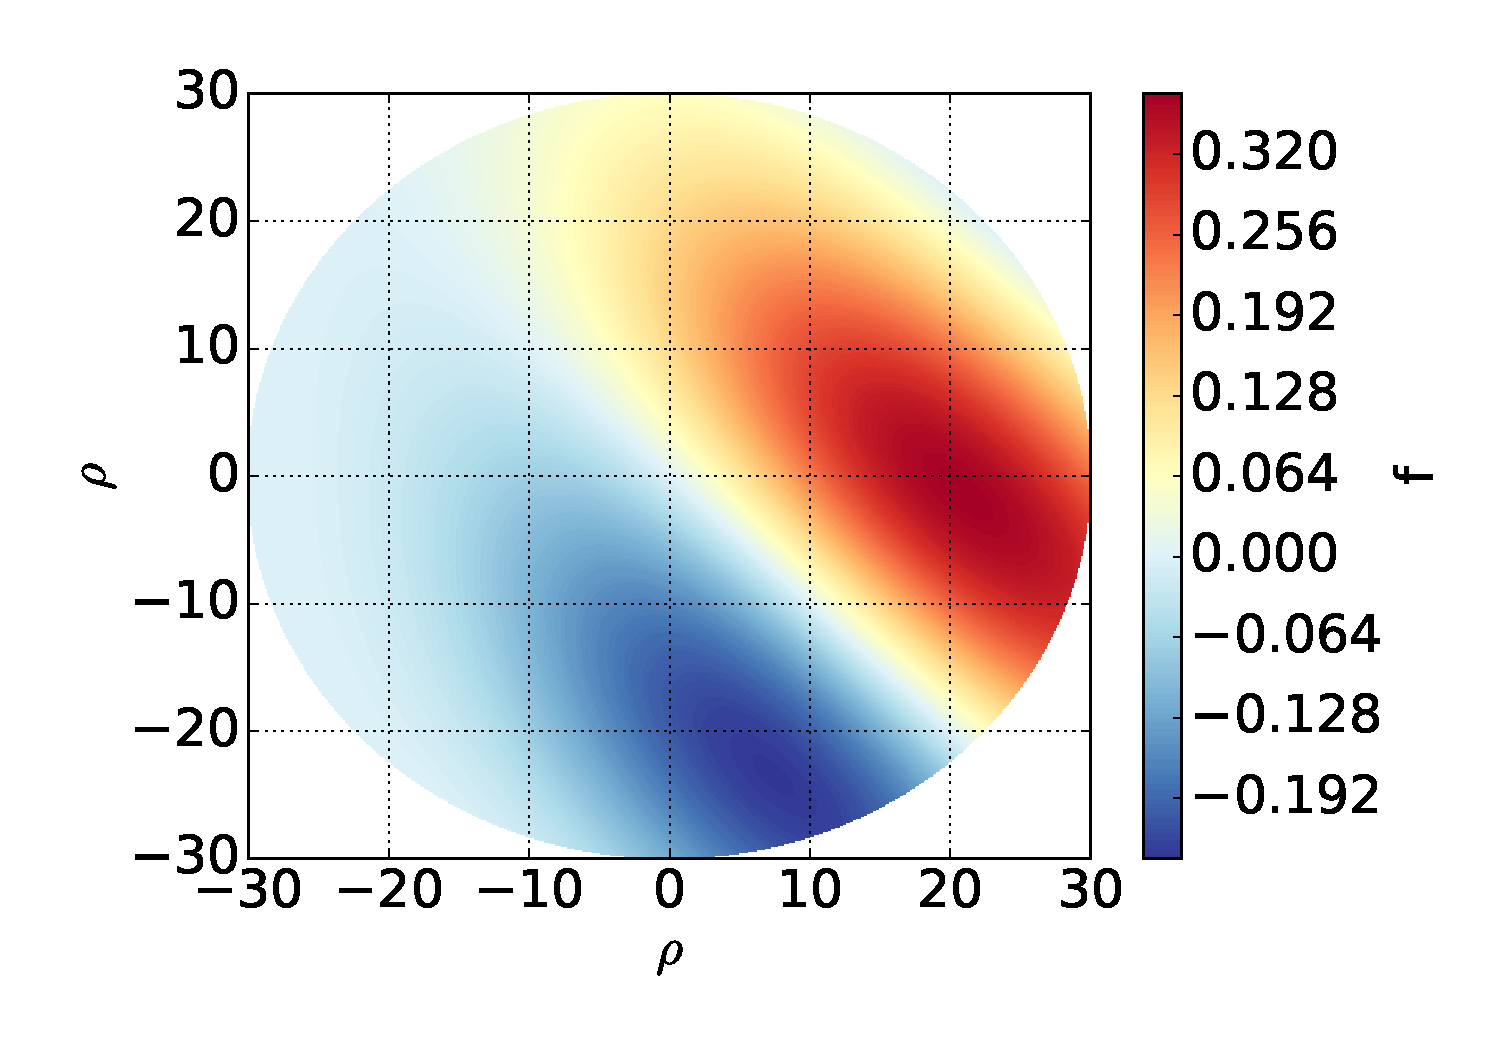
\includegraphics[width=1.0\textwidth]{fig/f}
        \caption{The function used in the MES}
    \end{subfigure}%
    ~
    \begin{subfigure}[t]{0.45\textwidth}
        \centering
        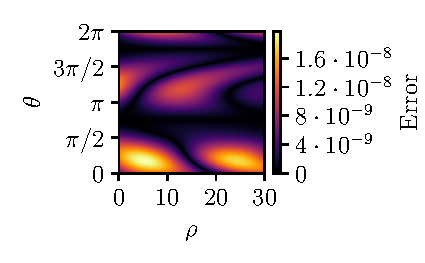
\includegraphics[width=1.0\textwidth]{fig/err}
        \caption{Typical plot of the errors}
    \end{subfigure}
    ~
    \begin{subfigure}[t]{0.45\textwidth}
        \centering
        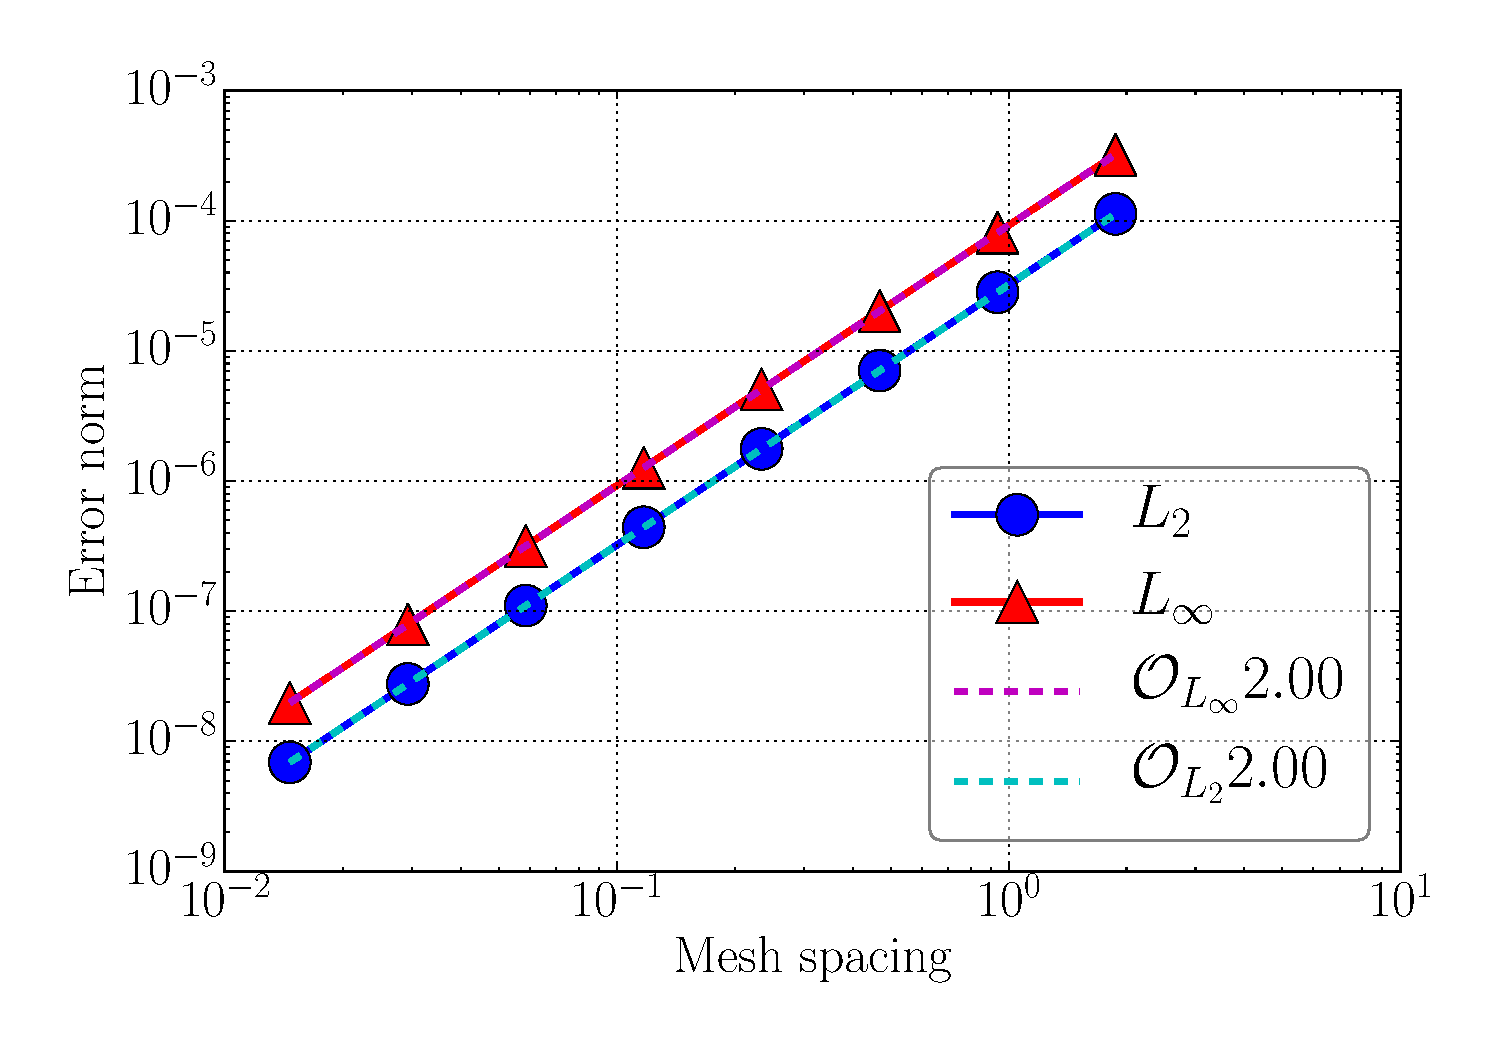
\includegraphics[width=1.0\textwidth]{fig/conv}
        \caption{Typical convergence plot}
    \end{subfigure}
    \caption{Typical function and errors for MES}
\end{figure}

\subsection{Single operators}
%
Although the single operators available from BOUT++ is verified in \cite{Dudson2016}, the axis of a cylinder must be treated with care as there is a singularity there ($J=0$ at $\rho=0$).
To overcome this problem the solution described in \cite{Naulin2008} has been used, and is illustrated in figure \ref{fig:innerRho}.
%
\begin{figure}[htb]
    \centering
    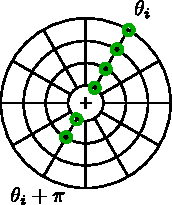
\includegraphics[width=0.3\textwidth]{fig/innerGhost}
    \caption{\textit{
        The green full circles represents the inner grid points at
        $\theta=\theta_i$. The green dashed circles at $\theta=\theta_i + \pi$
        are the ghost points (in the $\rho$-direction) belonging to the
        $\theta=\theta_i$ inner points. Equally the inner grid points at
        $\theta=\theta_i$ serves as ghost points (in the $\rho$-direction) for
        the inner points of $\theta=\theta_i + \pi$.
    }}
    \label{fig:innerRho}
\end{figure}
%
In this solution, the innermost ghost points%
\footnote{A grid point not belonging to the physical domain, but makes it possible to use a centered scheme when evaluating at the grid point closest to the physical boundary of the domain.}
in $\rho$ (closest to the singularity) with a $\theta$ value lower than (and excluding) $\pi$ will be set to the value of the innermost internal point%
\footnote{A grid point which is not a ghost points, i.e. it belongs to the physical domain.}%
%
which lies $\theta + \pi$ away.
The next ghost point will be set to the value of the second innermost internal point which lies $\theta + \pi$ away, and so on.
In this thesis, only one ghost point is used.

The convergence test for the single operators in $\rho$ direction can be found in table \ref{tb:singleRho}.
%
\begin{table}[h!]
{\footnotesize \centerline{
\begin{tabular}{c|llllp{3cm}}
\hline\hline
Operation & $L_\inf$ order & $L_2$ order &
$L_\inf$ error ($2^{12}$ points) & $L_2$ error ($2^{12}$ points) & Comment\\
\hline
$\texttt{DDX}  (f)$ & $2.00$ & $2.00$ & $1.99\cdot10^{-8}$ & $6.90\cdot10^{-9}$& \\
$\texttt{D2DX2}(f)$ & $2.00$ & $2.00$ & $1.58\cdot10^{-9}$ & $5.07\cdot10^{-10}$& \\
$\texttt{D3DX3}(f)$ & $1.73$ & $2.00$ & $9.66\cdot10^{-10}$ & $1.57\cdot10^{-9}$&
$L_\inf$ order $=2$ until $2^{11}$ points
\\
$\texttt{D2DXDZ} (f)$ & $2.00$ & $2.00$ & $1.09\cdot10^{-8}$ & $2.97\cdot10^{-8}$& \\
$\texttt{D3DX2DZ}(f)$ & $2.00$ & $1.94$ & $2.33\cdot10^{-9}$ & $8.51\cdot10^{-10}$&
$L_\inf$ order $=2$ until $2^{11}$ points
\\
$\texttt{D3DZ2DX}(f)$ & $2.00$ & $2.00$ & $7.68\cdot10^{-8}$ & $2.88\cdot10^{-8}$& \\
$\texttt{DDX}   (Jf)$ & $2.00$ & $2.00$ & $5.22\cdot10^{-7}$ & $1.71\cdot10^{-7}$& \\
$\texttt{DDX}(\texttt{DDX}[f])$ & $-1.00$ & $-0.50$ & $1.67\cdot10^{0}$ & $2.60\cdot10^{-2}$&
Solution diverges. Errors dominating close to $\rho=0$.
\\
$\frac{\texttt{DDX}(f)}{J}$ & $1.00$ & $1.50$ & $3.16\cdot10^{-5}$ & $4.48\cdot10^{-7}$&
No order $2$nd order convergence. Errors dominating close to $\rho=0$.
\\
\hline\hline
\end{tabular}
}}
\caption[]{\textit{Convergence test of single operators in the $\rho$ direction}}
\protect\label{tb:singleRho}
\end{table}
%
For the cases where a convergence order of $2$ is found up until $2^{11}$ points, the schemes are considered convergent as the error is not dominating at any particular point of the domain.
In general, one can observe from the plots of the error that they become a bit noisy in these cases, which could indicate that machine precision in reached.

Note in the two last cases in table \ref{tb:singleRho} that the converge one naively would have expected is generally not reached.
In the case where we use $\texttt{DDX}(\texttt{DDX}[f])$, the boundaries are reset after the first operation.
Notice that the resulting of stencil of these two operators is a wide stencil.
That is
%
\begin{align*}
D[D[f_i]] =& D\L[\frac{-f_{i-1} + f_{i+1}}{h_x}\R]
\\
=& \frac{-D[f_{i-1}] + D[f_{i+1}]}{h_x}
\\
=& \frac{-\frac{-f_{i-2} + f_{i}}{h_x} + \frac{-f_{i} + f_{i+2}}{h_x}}{h_x}
\\
=& \frac{f_{i-2} - 2f_{i} + f_{i+2}}{h_x^2}
\end{align*}
%
where $h_x$ denotes the grid spacing, and the subscript the grid index.
Hence, the observed divergence could be explained with poor information communication across the singularity.

In the case of $\frac{\texttt{DDX}(f)}{J}$, the loss of expected convergence rate can be explained by looking at the operator under investigation.
As the $\texttt{DDX}(f)$ operator used in this thesis is the standard $2$nd order operator (obtained by subtracting the function Taylor expanded around $x_0$, evaluated in $x+h$ from the function Taylor expanded around $x_0$, evaluated in $x-h$ and divided by $2h$), one find that
%
\begin{align*}
    \deri{f}{x} - \texttt{DDX}(f) =
    \frac{h^2}{6}\deri{^2f}{x^2} + \mathcal{O}(h^3)
\end{align*}
%
In the first inner point $J=h_x$ as the boundaries lays half between the grid points.
Thus, in this point, we have that
%
\begin{align*}
    \frac{ \L.\deri{f}{x} \R|_{\text{first} \rho}}{J}
    - \frac{\L. \texttt{DDX}(f)\R|_{\text{first} \rho}}{J}=
    \frac{h}{6}\deri{^2f}{x^2} + \mathcal{O}(h^2)
\end{align*}
%
Thus for the first inner point, the scheme is not $2$nd order convergent.

Only one extra operator is implemented in the $\theta$-direction.
This is shown in table \ref{tb:singleZ}.
Note that we use spectral methods in the $\theta$ direction, which is know to give minimal error.
Machine precision is therefore quickly reached, and performing MES after machine precision is nonsense due to loss of precision when subtracting two almost equal numbers.
Indications that machine precision is reached are low errors, and plots of the error appearing noisy
%
\begin{table}[h!]
{\footnotesize \centerline{
\begin{tabular}{c|llllp{3cm}}
\hline\hline
Operation & $L_\inf$ order & $L_2$ order &
$L_\inf$ error ($2^{6}$ points) & $L_2$ error ($2^{6}$ points) & Comment\\
\hline
\texttt{D3DZ3}$(f)$ & $2.06$ & $2.10$ & $7.44\cdot10^{-11}$ & $7.33\cdot10^{-12}$&
Reaches machine precision at $2^6$.
\\
\hline\hline
\end{tabular}
}}
\caption[]{\textit{Convergence test single operators in the $\theta$ direction.}}
\protect\label{tb:singleZ}
\end{table}

\subsection{Divergence operators}
%           ▸ 1a-divPerp/
%           ▸ 1b-JTimesDivPerp/
%           ▸ 2a-divSource/
%           ▸ 2b-JTimesDivSource/
%           ▸ 3a-divExBAdv/
%           ▸ 3b-J4divExBAdv/

\subsection{The Naulin Solver}
% FIXME: Write about the function
functions here
mention BC
write implementation somewhere
\begin{table}[h!]
{\footnotesize \centerline{
        \begin{tabular}{lllll}
\hline\hline
$L_\inf$ order & $L_2$ order &
$L_\inf$ error ($2^{12}$ points) & $L_2$ error ($2^{12}$ points)\\
\hline
$2.00$ & $2.00$ & $3.19\cdot10^{-7}$ & $1.65\cdot10^{-7}$\\
\hline\hline
\end{tabular}
}}
\caption[]{\textit{Convergence test of the Naulin Solver in the $\rho$ direction}}
\protect\label{tb:naulinSolver}
\end{table}
%          ▸ Naulinsolver0Bndry/

\subsection{Boundary conditions}
%          ▸ 1-yExtrapolation/
%          ▸ 2-uEParSheath/
%          ▸ 3-cauchyBC/
